Let us consider a $\triangle{ABC}$, and let $\vec{D}$,$\vec{E}$ and $\vec{F}$ be the mid- points of sides AB,BC and CA respectively.\\
Let us consider a line-segment joining the points $\vec{D}$ and $\vec{F}$ which are midpoints of line AB and CA.\\

\begin{figure}[!ht]
\centering
\resizebox{\columnwidth}{!}{
    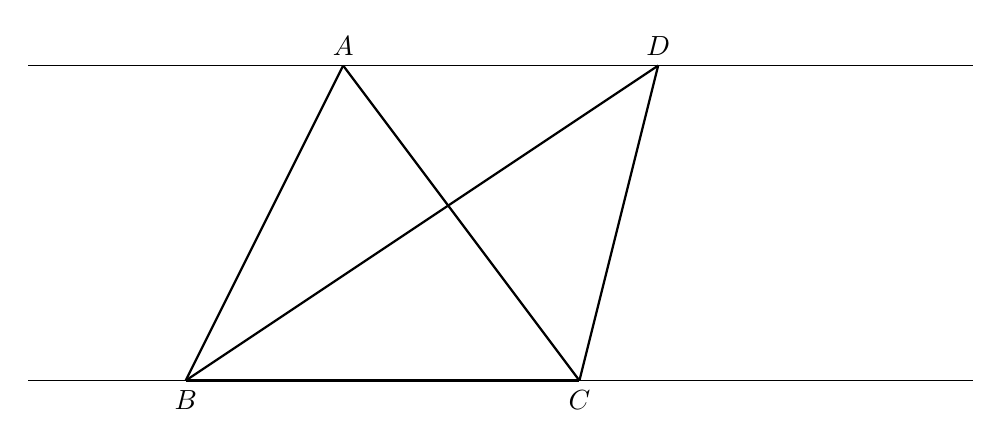
\begin{tikzpicture}
        \draw (-2,0) -- (10,0); 
        \draw (-2,4) -- (10,4);
        \filldraw[black] (0,0) node[anchor=north] {$B$};
        \filldraw[black] (2,4) node[anchor=south] {$A$};
        \filldraw[black] (5,0) node[anchor=north] {$C$};
        \filldraw[black] (6,4) node[anchor=south] {$D$};
        \draw[black,thick] (0,0) -- (2,4);
        \draw[black,thick] (0,0) -- (5,0);
        \draw[black,thick] (5,0) -- (2,4);
        \draw[black,thick] (0,0) -- (6,4);
        \draw[black,thick] (5,0) -- (6,4);
    \end{tikzpicture}}
\caption{Line segment DF joining mid-points of 2 sides of $\triangle{ABC}$}
\label{fig:solutions/5/tri_right_angle}
\end{figure}

As $\vec{D}$ is midpoint of line AB, $\vec{E}$ is midpoint of line BC and $\vec{F}$ is midpoint of line CA, they can be written as follows:
\begin{align}
    \vec{D}&=\frac{A+B}{2} \label{eq:solutions/5/mid_1}\\
    \vec{F}&=\frac{C+A}{2} \label{eq:solutions/5/mid_3}
\end{align}
The line DF can be written in the form of direction vector as,
\begin{equation} 
%\label{eq1}
\label{eq:solutions/5/res_1}
\begin{split}
\vec{m}_{DF}&=\vec{D}-\vec{F} \\
 &=\frac{A+B}{2}-\frac{C+A}{2}\\
 &=\frac{\vec{B}-\vec{C}}{2} \\
 &=\frac{\vec{m}_{BC}}{2}
\end{split}
\end{equation}
where $\vec{m}_{BC}$ is the direction vector of line BC.\\
Consider equation \eqref{eq:solutions/5/res_1},
\begin{align}
    \implies \vec{D}-\vec{F}&=\frac{\vec{B}-\vec{C}}{2}\label{eq:solutions/5/equa_2}
\end{align}
Applying norm on both sides of equation \eqref{eq:solutions/5/equa_2}, we get
\begin{align}
    \norm{\vec{D}-\vec{F}} = \frac{1}{2}\norm{\vec{B}-\vec{C}}\label{eq:solutions/5/res_2}
\end{align}\\
From equation\eqref{eq:solutions/5/res_1}, $\vec{DF}\parallel\vec{BC}$ and from \eqref{eq:solutions/5/res_2}, the line-segment $\vec{DF}=\frac{1}{2}\vec{BC}$

